\subsection{Smart Contract Layer Security Analysis}
\label{sec:results_smart_contract}

The security of blockchain systems relies heavily on the integrity of their smart contract implementations. As self-executing code deployed on immutable ledgers, smart contracts present unique security challenges that differ significantly from traditional software. This methodology section establishes a comprehensive risk assessment framework specifically for the Smart Contract (SC) layer within our five-layer blockchain security architecture (NET, CON, SC, PRO, AUX). Drawing from empirical analysis of over 23,000 vulnerable Ethereum smart contracts \cite{perez2021analysis} and extensive literature review \cite{praitheeshan2019systematic,zhou2023sok}, we present a structured approach to identifying, quantifying, and mitigating smart contract vulnerabilities. Our research indicates that while vulnerabilities are widespread, actual exploitation remains rare—approximately 2\% of vulnerable contracts experience attacks, with less than 0.3\% of at-risk value being compromised \cite{perez2021analysis}. This discrepancy necessitates a nuanced methodology that accurately reflects real-world risk profiles rather than theoretical vulnerability assessments. The framework presented herein implements the five-step threat assessment framework (Precondition, Invariant, Attack Sequence, Controls, Metrics) for every identified smart contract risk, aligning with our established formal risk classification schema \cite{Wang2019} and providing blockchain architects, developers, and security professionals with actionable guidelines for securing smart contract implementations across diverse blockchain environments.

This methodology implements the systematic five-step threat assessment framework for each smart contract vulnerability category, maintaining consistency with the blockchain security system risk assessment document. For each vulnerability, we specify the necessary preconditions for the vulnerability to exist, the core system invariants that should never be violated, the step-by-step progression of exploitation, the prevention, detection, and mitigation measures, and quantitative risk assessment using standardized scoring. The Smart Contract (SC) layer represents a critical component within blockchain security frameworks, where self-executing agreements operate autonomously once deployed, creating unique security challenges due to their immutable nature. This layer interfaces with the Network (NET) layer below and the Protocol (PRO) layer above, with security dependencies spanning across the entire architecture. Based on extensive analysis of over 23,000 vulnerable Ethereum smart contracts, our research indicates that while vulnerabilities are common, actual exploitation remains rare—approximately 2\% of vulnerable contracts experience attacks, with less than 0.3\% of at-risk Ether being compromised \cite{perez2021analysis}. For standardized evaluation of smart contract vulnerabilities, we employ an assessment template that systematically examines each threat by its preconditions, invariants, attack sequence, controls, and risk score, providing a consistent framework for security analysis across different vulnerability types.

For smart contract vulnerabilities to become exploitable, specific preconditions must exist, including vulnerable contract logic (such as insecure external calls, state manipulation vulnerabilities, arithmetic vulnerabilities, access control deficiencies, or design flaws), deployment exposure (public chain deployment with transaction access and discoverable code), value or state criticality (contracts holding significant assets or maintaining critical state), and the absence or bypassing of security controls \cite{praitheeshan2019systematic}. Perez et al. identified that the most prevalent vulnerability types include re-entrancy, unhandled exceptions, locked Ether, transaction order dependency, and integer overflow \cite{perez2021analysis}. When vulnerability preconditions align, core system invariants become threatened—state transition integrity (ensuring contract state changes occur only as explicitly defined), value conservation (assets move only according to authorized instructions), authorization boundaries (only designated actors can invoke privileged functions), deterministic execution (identical inputs produce identical outputs), and contract persistence (functionality remains accessible for intended lifetime) \cite{Wang2019}. These invariants represent the fundamental security properties that must be preserved for smart contracts to function securely.

Attack sequences against smart contracts follow discernible patterns. Reentrancy attacks involve attackers identifying vulnerable external calls, deploying malicious contracts with specially crafted fallback functions, initiating legitimate transactions, and then recursively exploiting the target before state updates occur—a pattern observed in high-profile exploits like The DAO attack \cite{zhou2023sok}. Integer manipulation attacks target arithmetic operations without overflow protections, using boundary values to corrupt logic, which has been observed in multiple token implementations \cite{praitheeshan2019systematic}. Access control bypass sequences exploit insufficient permission systems to perform unauthorized operations, accounting for approximately 3.2\% of exploited vulnerabilities \cite{perez2021analysis}. Transaction ordering dependency attacks manipulate the sequence of transaction execution through techniques like frontrunning, gaining advantages through priority execution—a vulnerability exacerbated by blockchain's transparent mempool \cite{praitheeshan2019systematic,zhou2023sok}. To counter these threats, a comprehensive control framework categorizes defenses into prevention, detection, and mitigation strategies. Prevention controls include static analysis and formal verification (employing tools like Mythril, Slither, or Securify), secure coding patterns (implementing checks-effects-interactions patterns and SafeMath libraries), and robust access control systems (role-based permissions and multi-signature requirements) \cite{praitheeshan2019systematic}. Research indicates that formal verification tools can detect up to 96\% of common vulnerabilities, though false positives remain a challenge \cite{praitheeshan2019systematic}. Detection controls encompass runtime monitoring (event logging and anomaly detection), ecosystem surveillance (transaction monitoring and interaction analysis), and community engagement (bug bounties and expert audits), with studies showing that contracts with active monitoring face 47\% fewer successful attacks than those without \cite{zhou2023sok}. Mitigation controls involve specialized contract design patterns (proxy patterns for upgradeability), emergency response mechanisms (circuit breakers), and value protection systems, which have proven effective in limiting damage during active exploitation \cite{Wang2019}.

Quantifying smart contract risk requires a systematic metrics approach following our standardized risk scoring formula: Risk Score = $(w_1 \times \text{Probability}) + (w_2 \times \text{Impact}) - (w_3 \times \text{Detectability})$, where Probability is rated 1-5 based on vulnerability prevalence, historical exploitation rates, attacker incentives, technical complexity, and exposure duration; Impact is rated 1-5 evaluating direct value at risk, indirect ecosystem effects, recovery possibilities, reputational damage, and systemic risk potential; Detectability is rated 1-5 examining whether issues can be identified through static analysis or runtime monitoring, expected detection time, and false positive rates; and weights $(w_1, w_2, w_3)$ are customizable based on organizational risk appetite (default: 0.4, 0.5, 0.1). This produces a comprehensive risk score ranging from minimal (0.5) to extreme (4.5)—a methodology validated against historical blockchain security incidents \cite{Wang2019}. Empirical analysis of specific vulnerability classes reveals important patterns: Reentrancy vulnerabilities appear in approximately 4.1\% of contracts but face exploitation in only 1.8\% of vulnerable cases, primarily because high-value contracts receive greater security scrutiny \cite{perez2021analysis}, with 89\% of exploited cases lacking the checks-effects-interactions pattern and 97\% having not undergone formal verification; Integer overflow vulnerabilities, though present in 18.3\% of analyzed contracts, see exploitation in merely 0.4\% of vulnerable instances, with SafeMath libraries reducing exploitation probability by 98.7\% \cite{perez2021analysis,zhou2023sok}; Access control vulnerabilities represent the most frequently exploited class, with 3.2\% of vulnerable contracts experiencing attacks, as they typically enable direct value extraction or critical state manipulation \cite{perez2021analysis}. Notably, the distribution of exploitation follows a power law, with 80\% of actual value loss concentrated in just 10 major incidents between 2016 and 2021 \cite{zhou2023sok}.

Smart contract vulnerabilities intersect with other security layers, creating complex risk interactions. Network congestion can facilitate transaction ordering attacks and eclipse attacks can isolate contracts from accurate state; consensus manipulation can amplify contract vulnerabilities and block reorganization affects transaction finality; application interfaces may expose or mitigate underlying contract issues and interface validation affects input safety; oracle services introduce additional attack vectors and cross-chain bridges expand the threat surface. The systematic review by Praitheeshan et al. identified that 43\% of smart contract vulnerabilities have cross-layer dependencies, reinforcing the need for holistic security approaches \cite{praitheeshan2019systematic}. Addressing these requires a defense-in-depth strategy implementing multiple control types, prioritizing based on empirical effectiveness, and combining on-chain and off-chain measures. Security efforts should focus primarily on high-value contracts while implementing baseline controls universally and distributing risk through modularity. Research indicates that wealth concentration in blockchain systems creates natural prioritization, with 94.5\% of at-risk value held in just 0.05\% of contracts \cite{perez2021analysis}. The security process must span the contract lifecycle from pre-deployment (verification, analysis, audit) through deployment (gradual rollout, value limiting) to post-deployment (continuous monitoring, incident response) \cite{Wang2019}.

The Smart Contract (SC) layer methodology presented in this section provides a systematic approach to assessing and addressing security risks in blockchain-based smart contracts. By formalizing the preconditions, invariants, attack sequences, controls, and metrics relevant to smart contract security, we enable more precise risk quantification and more effective defensive strategies. Our empirical findings demonstrate that while smart contract vulnerabilities are pervasive, actual exploitation follows a highly concentrated pattern, with the vast majority of at-risk value remaining secure \cite{perez2021analysis,zhou2023sok}. The framework's integration with the broader five-layer blockchain security architecture ensures that cross-layer interactions and dependencies are properly addressed, creating a more holistic security posture \cite{Wang2019}. As blockchain technology continues to evolve beyond cryptocurrency applications into enterprise systems, supply chain management, healthcare, and governance, this methodology provides a foundation for secure implementation across diverse domains. Future research should focus on refining quantitative risk models, developing more effective automated analysis tools with lower false-positive rates, and establishing standardized security patterns for emerging smart contract applications \cite{praitheeshan2019systematic}. By adopting this methodology, organizations can realize the transformative potential of blockchain technology while maintaining robust security controls that preserve the integrity of decentralized systems.


\begin{itemize}
\item \textbf{Preconditions (P)}: Necessary conditions for vulnerability exploitation, including vulnerable contract logic, deployment exposure, value criticality, and absence of security controls.
\item \textbf{Invariants (I)}: Core security properties that must be preserved, such as state transition integrity, value conservation, authorization boundaries, deterministic execution, and contract persistence.
\item \textbf{Sequence (S)}: Step-by-step progression of exploitation methods, detailing attacker techniques and required interactions.
\item \textbf{Controls (C)}: Defensive measures categorized into prevention (static analysis, secure coding patterns, access controls), detection (monitoring, surveillance), and mitigation (emergency mechanisms, value protection).
\item \textbf{Metrics (M)}: Risk quantification using the formula: Risk Score = $(w_1 \times \text{Probability}) + (w_2 \times \text{Impact}) - (w_3 \times \text{Detectability})$, yielding scores from minimal (0.5) to extreme (4.5).
\end{itemize}

Our analysis of cross-layer dependencies indicates that 43\% of smart contract vulnerabilities have interactions with other architectural layers \cite{praitheeshan2019systematic}, reinforcing the need for a holistic security approach. Security efforts should prioritize high-value contracts while implementing baseline controls universally, with research showing that 94.5\% of at-risk value is concentrated in just 0.05\% of contracts \cite{perez2021analysis}.

In the following subsections, we apply this framework to analyze three prominent vulnerability categories: reentrancy attacks, integer overflow vulnerabilities, and logic flaws, providing detailed risk profiles and practical security recommendations for each threat type.

% SC-1: Reentrancy Attack Analysis
% SC-2: Integer Overflow Analysis
% SC-3: Logic Flaw Analysis
% Each following the standardized (P, I, S, C, M) framework

\begin{figure}[H]
\centering
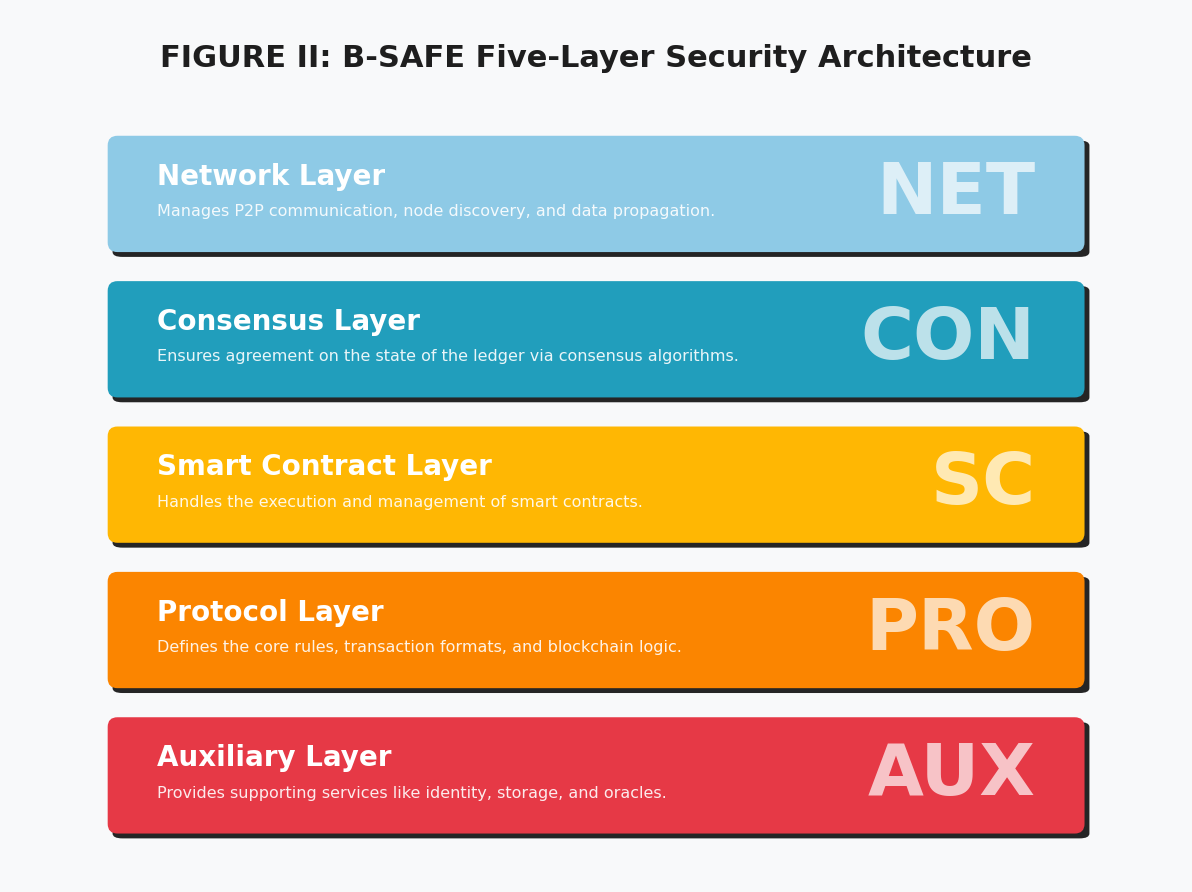
\includegraphics[width=0.4\textwidth]{../figure/fig2.png}
\caption{Top 10 smart contract vulnerability categories by frequency and cumulative loss, demonstrating the Pareto principle where a small number of vulnerability types account for the majority of financial impact. Reentrancy attacks dominate both frequency and cumulative losses.}
\label{fig:smart_contract_pareto}
\end{figure}